\documentclass[a4paper, 10pt]{article}

\author{Guillaume Cluzel}
\title{Toward a secure TCP/IP stack --- Technical report}

\usepackage{amsmath,amsfonts}

\usepackage{listings}

\lstset{
    basicstyle=\ttfamily
}

\usepackage{tikz}
\usetikzlibrary{calc,backgrounds,shapes}
\usetikzlibrary{arrows.meta, shapes.callouts}
\usetikzlibrary{decorations.pathreplacing}

\tikzset{global scale/.style={
    scale=#1,
    every node/.style={scale=#1}
  }
}

\usepackage{hyperref}

\usepackage[ruled]{algorithm2e}

\usepackage[backend=biber]{biblatex}
\addbibresource{biblio.bib}

\DeclareMathOperator{\Pre}{Pre}
\DeclareMathOperator{\Post}{Post}

\let\state\textsf
\newcommand\ESTABLISHED{\state{ESTABLISHED}}
\newcommand\SYNRECEIVED{\state{SYN-RECEIVED}}
\newcommand\CLOSED{\state{CLOSED}}
\newcommand\CLOSEWAIT{\state{CLOSE-WAIT}}
\newcommand\LISTEN{\state{LISTEN}}
\newcommand\SYNSENT{\state{SYN-SENT}}
\newcommand\FINWAITONE{\state{FIN-WAIT-1}}
\newcommand\FINWAITTWO{\state{FIN-WAIT-2}}
\newcommand\CLOSING{\state{CLOSING}}
\newcommand\LASTACK{\state{LAST-ACK}}
\newcommand\TIMEWAIT{\state{TIME-WAIT}}

\begin{document}

    \maketitle

    \tableofcontents

    \section{Introduction}

    TCP is a widely used network protocol to communicate in the Internet as
    it is used by the HTTP protocol, the FTP protocol, and so many others.
    Ensuring the safety of the TCP/IP stack is essential for the safety of
    a lot of machines. While a lot of work has been done on formally verifying higher level
    protocols, such as SSL/TLS which is built on top of TCP and designed
    to provide a security layer to TCP with for example the work done in
    miTLS~\cite{bhargavan2013implementing}, or at a lower level with the work
    on RecordFlux to safely parse data segments~\cite{Reiher_2020}, nothing has
    been done to formally verify a secure TCP implementation. However, TLS security
    can only be ensured if the underlying TCP implementation is free of bugs.

    CycloneTCP is a library developed by the company Oryx Embedded for embedded platforms.
    A large number of platforms are supported, and the library can be used
    with a dozen of OS. The code of the library is written in C and implements
    many protocols from low-level network layers like IPv4/IPv6, to transport layers
    and application layers like DHCP or HTTP. In particular an implementation of
    the TCP protocol is provided.

    SPARK 2014 is a programming language designed as a subset of Ada that helps in
    making high reliability software by providing powerful static analysis methods.
    SPARK is able to detect uninitialized variables with control flow analysis,
    and can ensure the absence of run-time errors,
    but also, based on SMT-solver, functional behavior can be specified for every
    function and mathematically proved.

    The aim of this work was to translate some parts of the CycloneTCP TCP/IP stack
    in Ada/SPARK to improve the safety of the code. In particular we focused
    on the TCP protocol to ensure that the norm is respected in the code.

    This report is a synthesis of the challenge of verifying such a protocol
    and the solution we found during the internship to go towards a secure protocol.


    \section{The TCP protocol}

    \subsection{Why verify a TCP stack?}

    As mentioned in the introduction, TCP protocol is the base of a lot of other protocols,
    in particular SSL/TLS. These higher protocols cannot be secure if the underlying TCP protocol
    has bugs. An incorrect implementation of the TCP protocol can lead to a crash
    in the communication if two machines cannot communicate together, to an error in
    retransmissions, or even to security failures. CycloneTCP is designed for embedded
    code, and a failure in the code can be critical.


    \subsection{Sockets}

    A socket is nothing more than a data structure that contains the connection
    information, like for example the local or the remote IP address as well as
    the state of the connection and other information required by the TCP protocol.
    In Ada, a socket will be represented by a pointer to a record type:

    \begin{lstlisting}[language=Ada]
type Socket_Struct is record
    S_Descriptor     : Sock_Descriptor;
    S_Type           : Socket_Type;
    S_Protocol       : Socket_Protocol;
    S_Net_Interface  : System.Address;
    S_localIpAddr    : IpAddr;
    S_Local_Port     : Port;
    S_Remote_Ip_Addr : IpAddr;
    S_Remote_Port    : Port;
    S_Timeout        : Systime;
    State            : Tcp_State;
    -- Other fields
end record;
type Socket is access Socket_Struct;
    \end{lstlisting}

    A socket is also the structure that is manipulated by the users as an opaque structure,
    through an API to perform operations on the socket itself and on the
    global environment by sending messages in the network for example.

    \subsection{Presentation of the protocol}

    TCP is defined by the norm RFC 793 \cite{rfc793} in a high level language.
    TCP is a reliable, ordered and error-checked connection oriented protocol.
    It means that two computers have to open a connection first before sending data.
    The connection is closed once all the data has been transmitted.
    The flow of a connection (if no error happens) contains three main steps:
    \begin{enumerate}
        \item Opening the connection,
        \item Sending \& receiving the data,
        \item Closing the connection.
    \end{enumerate}

    This mechanism is decribed by a state machine.

    \begin{figure}[p]
        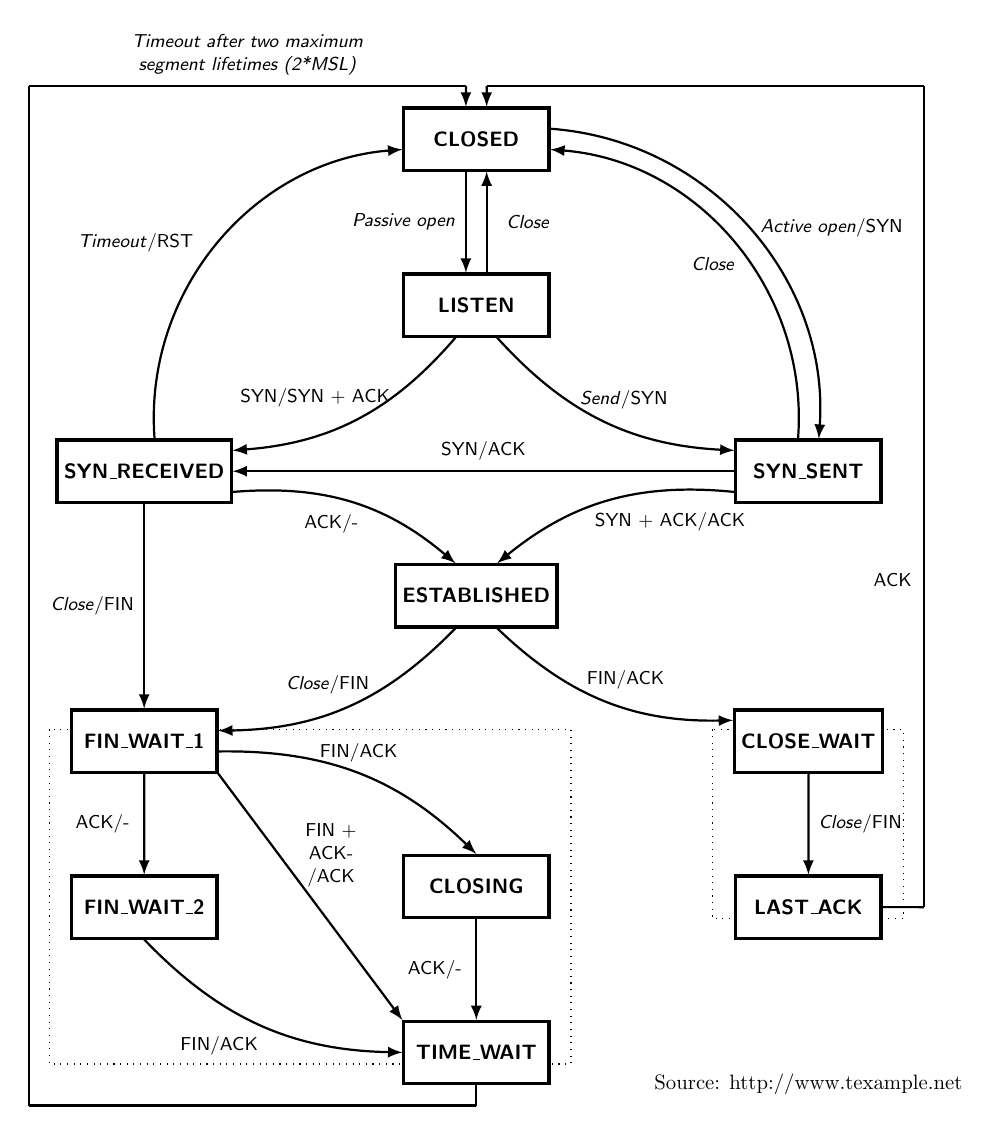
\begin{tikzpicture}[>=latex, global scale=.75]
            
        %
        % Styles for states, and state edges
        %
        \tikzstyle{state} = [draw, very thick, fill=white, rectangle, minimum height=3em, minimum width=7em, node distance=8em, font={\sffamily\bfseries}]
        \tikzstyle{stateEdgePortion} = [black,thick];
        \tikzstyle{stateEdge} = [stateEdgePortion,->];
        \tikzstyle{edgeLabel} = [pos=0.5, text centered, font={\sffamily\small}];
        
        %
        % Position States
        %
        \node[state, name=closedStart] {CLOSED};
        \node[state, name=listen, below of=closedStart] {LISTEN};
        \node[state, name=synSent, below of=listen, right of=listen, xshift=8em] {SYN\_SENT};
        \node[state, name=synRcvd, below of=listen, left of=listen, xshift=-8em] {SYN\_RECEIVED};
        \node[state, name=established, below of=listen, node distance=14em] {ESTABLISHED};
        \node[state, name=finWait1, below of=established, left of=established, node distance=7em, xshift=-9em] {FIN\_WAIT\_1};
        \node[state, name=finWait2, below of=finWait1] {FIN\_WAIT\_2};
        \node[state, name=closeWait, below of=established, right of=established, node distance=7em, xshift=9em] {CLOSE\_WAIT};
        \node[state, name=closing, below of=established, node distance=14em] {CLOSING};
        \node[state, name=lastAck, below of=closeWait] {LAST\_ACK};
        \node[state, name=timeWait, below of=closing] {TIME\_WAIT};
        
        \node at ($(lastAck) + (0,-3)$) {Source: \url{http://www.texample.net}};
        
        %
        % Connect States via edges
        %
        \draw ($(closedStart.south) + (-.5em,0)$) 
        edge[stateEdge] node[edgeLabel, xshift=-3em]{\emph{Passive open}} 
        ($(listen.north) + (-.5em,0)$); 
        \draw ($(listen.north) + (.5em,0)$) 
        edge[stateEdge] node[edgeLabel, xshift=2em]{\emph{Close}} 
        ($(closedStart.south) + (.5em,0)$);
        
        \draw ($(listen.south) + (-1em,0)$) 
        edge[stateEdge, bend left=22.5] node[edgeLabel, xshift=-2em, yshift=1em]{SYN/SYN + ACK} 
        ($(synRcvd.east) + (0,1em)$);
        \draw ($(listen.south) + (1em,0)$) 
        edge[stateEdge, bend right=22.5] node[edgeLabel, xshift=1em, yshift=1em]{\emph{Send}/SYN} 
        ($(synSent.west) + (0,1em)$);
        
        \draw ($(synRcvd.north) + (.5em,0)$) 
        edge[stateEdge, bend left=45] node[edgeLabel,xshift=-4em]{\emph{Timeout}/RST} 
        ($(closedStart.west) + (0,-.5em)$);
        
        \draw ($(synSent.north) + (-.5em,0)$) 
        edge[stateEdge, bend right=45] node[edgeLabel,xshift=-1em, yshift=-1em]{\emph{Close}} 
        ($(closedStart.east) + (0,-.5em)$);
        \draw ($(closedStart.east) + (0,.5em)$) 
        edge[stateEdge, bend left=45] node[edgeLabel,xshift=4em]{\emph{Active open}/SYN} 
        ($(synSent.north) + (.5em,0)$);
        
        \draw (synSent.west) 
        edge[stateEdge] node[edgeLabel, yshift=1em]{SYN/ACK} 
        (synRcvd.east);
        \draw (synRcvd) 
        edge[stateEdge] node[edgeLabel, xshift=-2.5em]{\emph{Close}/FIN} 
        (finWait1);
        
        \draw ($(synRcvd.east) + (0,-1em)$) 
        edge[stateEdge, bend left=22.5] node[edgeLabel, xshift=-1em, yshift=-1em]{ACK/-} 
        ($(established.north) + (-1em,0)$);
        \draw ($(synSent.west) + (0,-1em)$) 
        edge[stateEdge, bend right=22.5] node[edgeLabel, xshift=3em, yshift=-1em]{SYN + ACK/ACK} 
        ($(established.north) + (1em,0)$);
        
        \draw ($(established.south) + (-1em,0)$) 
        edge[stateEdge, bend left=22.5] node[edgeLabel, xshift=-1em, yshift=1em]{\emph{Close}/FIN} 
        ($(finWait1.east) + (0,.5em)$);
        \draw ($(established.south) + (1em,0)$) 
        edge[stateEdge, bend right=22.5] node[edgeLabel, xshift=1em, yshift=1em]{FIN/ACK} 
        ($(closeWait.west) + (0,1em)$);
        
        \draw (finWait1.south) 
        edge[stateEdge] node[edgeLabel, xshift=-2em]{ACK/-} 
        (finWait2.north);
        \draw ($(finWait1.east) + (0,-.5em)$) 
        edge[stateEdge, bend left=22.5] node[edgeLabel, yshift=1em]{FIN/ACK} 
        (closing.north);
        \draw (finWait1.south east) 
        edge[stateEdge] node[edgeLabel, xshift=1em, yshift=2em, text width=3em]{FIN + ACK/ACK} 
        (timeWait.north west);
        
        \draw (finWait2.south) 
        edge[stateEdge, bend right=22.5] node[edgeLabel, xshift=-2em, yshift=-1em]{FIN/ACK} 
        (timeWait.west);
        
        \draw (closing) 
        edge[stateEdge] node[edgeLabel, xshift=-2em]{ACK/-} 
        (timeWait);
        
        \draw (closeWait) 
        edge[stateEdge] node[edgeLabel,xshift=2.5em]{\emph{Close}/FIN} 
        (lastAck);
        
        %
        % Connect lastAck to closed is slightly more complicated
        % no direct line-of-sight, so we need to take the scenic route
        %
        \coordinate (lastAck2ClosedA) at ($(lastAck.east) + (2em,0)$);
        \coordinate (lastAck2ClosedB) at ($(closedStart.north -| lastAck.east) + (2em,1em)$);
        \coordinate (lastAck2ClosedC) at ($(closedStart.north) + (0.5em,1em)$);
        \draw (lastAck.east) edge[stateEdgePortion] (lastAck2ClosedA);
        \draw (lastAck2ClosedA) edge[stateEdgePortion] node[edgeLabel,xshift=-1.5em, yshift=-4em]{ACK} (lastAck2ClosedB);
        \draw (lastAck2ClosedB) edge[stateEdgePortion] (lastAck2ClosedC);
        \draw (lastAck2ClosedC) edge[stateEdge] ($(closedStart.north) + (0.5em,0)$);
        
        %
        % likewise for timeWait to closed
        %
        \coordinate (timeWait2ClosedA) at ($(timeWait.south) + (0,-1em)$);
        \coordinate (timeWait2ClosedB) at ($(timeWait.south -| finWait2.west) + (-2em,-1em)$);
        \coordinate (timeWait2ClosedC) at ($(closedStart.north -| finWait2.west) + (-2em,1em)$);
        \coordinate (timeWait2ClosedD) at ($(closedStart.north) + (-0.5em,1em)$);
        \draw (timeWait.south) edge[stateEdgePortion] (timeWait2ClosedA);
        \draw (timeWait2ClosedA) edge[stateEdgePortion] (timeWait2ClosedB);
        \draw (timeWait2ClosedB) edge[stateEdgePortion] (timeWait2ClosedC);
        \draw (timeWait2ClosedC) edge[stateEdgePortion] 
        node[edgeLabel, text width=12.25em, yshift=1.5em]{\emph{Timeout after two maximum segment lifetimes (2*MSL)}} 
        (timeWait2ClosedD);
        \draw (timeWait2ClosedD) edge[stateEdge] ($(closedStart.north) + (-0.5em,0)$);
        
        % draw dotted lines around passive and active closes
        \begin{pgfonlayer}{background}
            \draw [join=round,black,dotted] ($(closeWait.north west) + (-1em, -1em)$) rectangle ($(lastAck.south east) + (1em, 1em)$);
            \draw [join=round,black,dotted] ($(finWait1.north west) + (-1em, -1em)$) rectangle ($(timeWait.south east) + (1em, 1em)$);
        \end{pgfonlayer}
        
        \end{tikzpicture}
        \caption{TCP automaton.}
        \label{fig:TCPAutomaton}
    \end{figure}

    As it can be seen in the state machine diagram in figure \ref{fig:TCPAutomaton},
    a socket can take different states that are
    subject to change when a message (or a segment) is sent or received or when an action
    is performed by the user. A label $A/B$ on an edge in the graph refers to a stimulus performed on the socket
    (the reception of a message, a user action...) for $A$ and a flag sent for $B$.
    More precisely, for $A$, a text in italic shape refers to an action performed by
    the user (a call of a user function) or when it's a timeout the action is automatically
    performed by a timer, and a ACK, SYN or FIN refers to a flag contained in a received message.
    The flags in $B$ refer to the flags sent in response of the stimulus by $A$.
    Without giving unnecessary details on the format of a TCP header, we can
    describe some flags that can be contained in a TCP header in order to help the understanding
    of figure \ref{fig:TCPAutomaton}:
    \begin{description}
        \item[ACK] Acknowledgment field significant. The last message received by the sender
        is acknowledged. A field of the header contains the number of this segment.
        \item[SYN] Synchronize sequence number. This flag is sent in order to establish
        a connection.
        \item[FIN] No more data from sender. This flag is sent in order to close the
        connection.
    \end{description}
    
    Different states can be taken by a socket during its lifetime depending on the state
    of the connection. The state also gives information about the state of the remote TCP.
    Each state has its own signification:
    \begin{description}
        \item[\CLOSED] represents no connection state at all.
        \item[\LISTEN] represents waiting for a connection request from any remote
        TCP and port.
        \item[\SYNSENT] represents waiting for a matching connection request
        after having sent a connection request.
        \item[\SYNRECEIVED] represents waiting for a confirming connection
        request acknowledgment after having both received and sent a
        connection request.
        \item[\ESTABLISHED] represents an open connection, data received can be
        delivered to the user. The normal state for the data transfer phase
        of the connection.
        \item[\FINWAITONE{}] represents waiting for a connection termination request
        from the remote TCP, or an acknowledgment of the connection
        termination request previously sent.
        \item[\FINWAITTWO{}] represents waiting for a connection termination request
        from the remote TCP.
        \item[\CLOSEWAIT] represents waiting for a connection termination request
        from the local user.
        \item[\CLOSING{}] represents waiting for a connection termination request
        acknowledgment from the remote TCP.
        \item[\LASTACK{}] represents waiting for an acknowledgment of the
        connection termination request previously sent to the remote TCP
        (which includes an acknowledgment of its connection termination
        request).
        \item[\TIMEWAIT{}] represents waiting for enough time to pass to be sure
        the remote TCP received the acknowledgment of its connection
        termination request.
    \end{description}

    \paragraph{Example of a possible way to establish a connection}

    We present a scenario on how a connection can be established between two TCPs,
    when one TCP (TCP A) is in the state \CLOSED{} and the other (TCP B) is in the state \LISTEN.
    \begin{enumerate}
        \item TCP A wants to initiate a connection with TCP B. It sends a SYN segment to
            TCP B and passes to the state \SYNSENT{}.

        \item TCP B receives a segment SYN. It has to respond to this segment by a segment
            containing the flags SYN and ACK (acknowledgment of the received segment).
            It changes its state for \SYNRECEIVED. 

        \item When TCP A receives the segment sent by TCP B containing the flags SYN and ACK,
            it only has to send back an ACK of this segment to pass in the state \ESTABLISHED.

        \item TCP B receives the ACK of its segment and pass in state \ESTABLISHED{} too.
    \end{enumerate}
    At the end of this procedure, the two TCPs are in state \ESTABLISHED{} and can start to
    send data. Figure \ref{fig:handshake} illustrates the procedure described above. This procedure to open a connection is known as the ``three-way
    handshake'' in the TCP norm.

    \begin{figure}
        \centering
        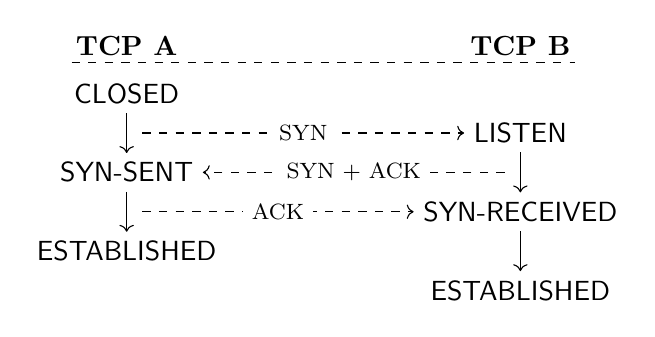
\begin{tikzpicture}
            \node (A) at (0, 5) {\bfseries TCP A};
            \node (B) at (5, 5) {\bfseries TCP B};
            \draw[dashed] (-.7,4.8) -- (5.7,4.8);
            \node (TCPA1) at (0, 4.4) {\CLOSED{}};
            \node (TCPB1) at (5, 3.9) {\LISTEN{}};
            \node (TCPA2) at (0, 3.4) {\SYNSENT};
            \node (TCPB2) at (5, 2.9) {\SYNRECEIVED{}};
            \node (TCPA3) at (0, 2.4) {\ESTABLISHED{}};
            \node (TCPB3) at (5, 1.9) {\ESTABLISHED{}};

            \draw[->] (TCPA1) -- (TCPA2);
            \draw[->] (TCPB1) -- (TCPB2);
            \draw[->] (TCPA2) -- (TCPA3);
            \draw[->] (TCPB2) -- (TCPB3);
            \draw[->, dashed] (0.2, 3.9) -- node [midway, fill=white] {\footnotesize SYN} (TCPB1);
            \draw[->, dashed] (4.8, 3.4) -- node [midway, fill=white] {\footnotesize SYN + ACK} (TCPA2);
            \draw[->, dashed] (0.2, 2.9) -- node [midway, fill=white] {\footnotesize ACK} (TCPB2);
        \end{tikzpicture}
        \par
        \caption{Three-way hanshake procedure. The solid lines represent the transition between
        the states and the dashed lines represent the messages sent.}
        \label{fig:handshake}
    \end{figure}


    \bigskip

    We want to point out to the reader the differences that exist between the state machine
    of figure \ref{fig:TCPAutomaton} and the one that can be found in~\cite[23]{rfc793}. In particular
    a transition between the states \FINWAITONE{} and \TIMEWAIT{} has been added. It reflects the case where
    the ACK and FIN flags are received in the same segment. It is an allowed behavior by the norm, and
    also it is closer to what is done in CycloneTCP library.

    For more details on how two TCPs can establish or close a connection, the reader can refer
    to the TCP norm where many scenarios are described and explained, and more
    details are given on the state and segments that can be sent.


    \subsubsection{Multitasking in the implementation}

    Different tasks can interact with a socket. The TCP norm gives an example with
    three tasks: one for the \emph{user calls}, one for the \emph{arriving segments}
    and one for the \emph{timers}. This design has also been adopted in CycloneTCP.
    
    \paragraph{User calls}
    User calls refer to functions that can be called by the user to control the connection,
    send, or receive data: OPEN, CLOSE, ABORT, SEND, RECEIVED. Transition between states of
    the connection can happen during the call of these functions since they are intended to control
    the connection.

    \paragraph{Arriving segments}
    In this task, the received segments are processed. The corresponding messages are sent back.
    Transitions between states can happen here when a message is received. For example,
    this is the case when a message containing a SYN is received when the socket is in
    the \LISTEN{} state. It will automatically send a SYN + ACK in response, and change
    its state for \SYNRECEIVED.

    \paragraph{Timers}
    The timers control the timeouts like the retransmission timeout to retransmit a message, or
    the time-wait timeout to close the connection after an amount of time. Then, transitions can also
    happen in this task.

    To sum up, a single socket can be seen as a shared structure over multiple tasks, that can all
    manipulate it and change the value of its fields. The schema in figure \ref{fig:TCPConcurrency} illustrates that.
    
    Only one task can perform an operation on the socket at the same time. The access to the fields of
    the socket are protected by mutex.

    Two tasks can communicate synchronously or asynchronously together. The synchronous communications are based on
    the interface provided by the OS, in particular with events.

    \begin{figure}
        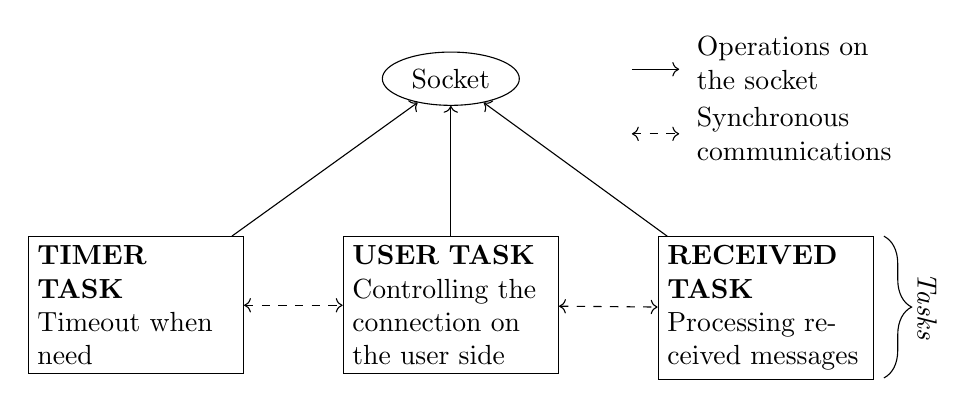
\begin{tikzpicture}
            \node [draw, ellipse] (S) at (2, 2) {Socket};
            \node [draw, text width=2.5cm, anchor=north] (T1) at (-2,0) {\textbf{TIMER TASK} \\
                                                    Timeout when need};
            \node [draw, text width=2.5cm, anchor=north] (T2) at (2,0) {\textbf{USER TASK} \\
                                                    Controlling the connection on the user side};
            \node [draw, text width=2.5cm, anchor=north] (T3) at (6, 0) {\textbf{RECEIVED TASK} \\
                                                    Processing received messages};
            \draw[->] (T1) -- (S);
            \draw[->] (T2) -- (S);
            \draw[->] (T3) -- (S);
            \draw[<->, dashed] (T1) -- (T2);
            \draw[<->, dashed] (T2) -- (T3);

            \draw[decorate, decoration={brace, amplitude=10pt}] (7.5, 0) -- (7.5, -1.8)
                node [black,midway,xshift=0.55cm, rotate=-90] {\textit{Tasks}};

            \draw [->] (4.3,2.12) -- (4.9,2.12);
            \node [anchor=west, text width=2.7cm] at (5,2.2) {Operations on the socket};
            \draw[<->, dashed] (4.3,1.3) -- (4.9,1.3);
            \node [anchor=west, text width=2.7cm] at (5, 1.3) {Synchronous communications};
        \end{tikzpicture}
        \caption{Concurrency in the TCP protocol.}
        \label{fig:TCPConcurrency}
    \end{figure}


    \section{Challenges}

    \subsection{Main focus for the verification}

    The TCP norm defines a lot of behavior that could be verified by automatic proof.
    Here is a non exhaustive list of what could be done:
    \begin{itemize}
        \item Verification of the transitions between the states.
        \item Integrity of the messages sent, \textit{i.e.} we could check that the sent
        message contains the correct flag and the correct sequence and acknowledgment numbers.
        \item Integrity of the messages received, \textit{i.e.} we could check that the
        messages received are correctly processed in regard of the flags they contain.
        \item Functional correctness of the user functions in regard to their specifications.
    \end{itemize}

    Some choices have had to be made in regard to the short time devolved to the internship, and
    not every aspect of the TCP norm has been proved yet. However, some aspects have been selected
    for the challenge or the importance they represent. A list of these aspects is presented
    here and the choices will be motivated in the next subsections. First of all, we have wanted
    to improve the interface of the functions. The other point was to improve the safety of the
    protocol itself.

    \subsubsection{Improve the functional interface}

    One of the main problems pointed to by the main author of the CycloneTCP library is that users
    do not correctly use the API supplied. As a result, some function
    calls can be incorrect, either because the arguments are incorrect, or because the
    return code of the previous calls has not been checked, which leads to an
    incorrect code.

    \subsubsection{Respect of the protocol}

    To ensure the safety of the library, it is necessary to ensure that the functions really
    do what they are supposed to do. It is a part of the job that has been done. More
    especially we have wanted to check if the state machine is respected by all the
    user functions in the transition they do. We have also tried to ensure the correctness
    of the functions called regarding the TCP state of the socket before the call
    to respect the specifications given in the norm.


    \subsection{Technical problems encountered}

    The multiple tasks and the changes that can happen at every moment in one
    task or another make the verification hard. Multiple interactions exist
    between the multiple tasks: synchronous and asynchronous.
    All these interactions have to be considered if we want to write correct contracts
    in regard to what could be done in other tasks.

    As SPARK does not have a native mode to deal precisely with interactions related to concurrency, we have to
    model these different interactions by hands by writing assertions that
    modify the state of the socket as another task could do it. In particular
    the problem has been encountered when we tried to write contracts for the correctness
    of the user functions. More details and explanations will be given in the following
    section, where we will investigate the solution found to these technical problems.

    \section{Solutions found}

    \subsection{Order to call the functions}

    This part mainly focuses on the high level user functions, the socket functions.
    The socket functions are the one called by the user to perform operations on
    the network. They are located in the files \texttt{socket\_interface.ad(b|s)}.

    It is clear that there exists an order in which the functions have to be called.
    This order can be determined by the norm, and must respect the order given by the
    graph in figure \ref{fig:TCPAutomaton}.
    Then, we want post- and pre-conditions to model a partial order on the calls of the function.
    If two functions $f_1$ and $f_2$ are ordered such that $f_1 \preceq f_2$ where $\preceq$ is
    a relation over the order in which functions have to be called, then we want that the
    post-condition of $f_1$ implies the precondition of $f_2$, \textit{i.e.} $\Pre(f_2) \subseteq \Post(f_1)$.
    
    We will give an example over functions \lstinline[language=Ada]{Socket_Connect} and
    \lstinline[language=Ada]{Socket_Send}. The function \lstinline[language=Ada]{Socket_Connect}
    tries to connect to a distant TCP. If the connection succeeds, the remote IP address of the distant
    TCP is set in the field \lstinline[language=Ada]{S_Remote_Ip_Addr} of the \lstinline[language=Ada]{Sock}
    structure. When a user calls the function \lstinline[language=Ada]{Socket_Send}, we want to ensure that
    the connection has already been established. This is why a precondition of this function is
    \lstinline[language=Ada]{Is_Initialized_Ip(Sock.S_Remote_Ip_Addr)}. This precondition will only
    be proved if \lstinline[language=Ada]{Socket_Connect} has been previously called.


    \begin{figure}
        \begin{lstlisting}[language=Ada]
procedure Socket_Connect
    (Sock           : in out Not_Null_Socket;
     Remote_Ip_Addr : in     IpAddr;
     Remote_Port    : in     Port;
     Error          :    out Error_T)
  with
   Pre => Is_Initialized_Ip (Remote_Ip_Addr),
   Contract_Cases => (
     Sock.S_Type = SOCKET_TYPE_STREAM =>
       (if Error = NO_ERROR then
         Sock.S_Type = Sock.S_Type'Old and then
         Sock.S_Protocol = Sock.S_Protocol'Old and then
         Is_Initialized_Ip (Sock.S_localIpAddr) and then
         Sock.S_Local_Port = Sock.S_Local_Port'Old and then
         Sock.S_Remote_Ip_Addr = Remote_Ip_Addr and then
         Sock.S_Remote_Port = Remote_Port and then
         Sock.State = TCP_STATE_ESTABLISHED
       else
         Sock.S_Type = Sock.S_Type'Old and then
         Sock.S_Protocol = Sock.S_Protocol'Old)
     others => True)

procedure Socket_Send
    (Sock    : in out Not_Null_Socket;
     Data    : in     Send_Buffer;
     Written :    out Natural;
     Flags   :        Socket_Flags;
     Error   :    out Error_T)
  with
   Pre  =>
     Is_Initialized_Ip(Sock.S_Remote_Ip_Addr)
        \end{lstlisting}
        \caption{An example of how function calls can be ordered by Pre- and Post-conditions.}
        \label{code:FunOrdered}
    \end{figure}

    \subsection{Check of return code}

    An observation made by Clément Zeller, the main programmer of the library is that customers
    do not always think to check the return code of the socket user functions, to deal with the
    possibility that the call fails.
    If the return code is not checked, some assumption on the result cannot be done.

    The post-conditions as we have written them in SPARK, ensure that the return code is checked
    before processing continues. Figure \ref{code:FunOrdered} shows this mechanism for the
    procedure \lstinline[language=Ada]{Socket_Connect}. The post-condition distinguishes the cases
    where \lstinline{Error} is \lstinline{NO_ERROR} and where \lstinline{Error} takes another value.
    As a result, a user who would write an incorrect code such as
    \begin{lstlisting}[language=Ada]
    Socket_Connect (Sock, Remote_Ip_Addr, Port, Error);
    Socket_Send (Sock, Data, Written, Flags, Error);
    \end{lstlisting}
    would be warned by gnatprove with a message such as
    \begin{verbatim}
    medium: precondition might fail.
    \end{verbatim}
    whereas the following code is correct
    \begin{lstlisting}[language=Ada]
    Socket_Connect (Sock, Remote_Ip_Addr, Port, Error);
    if Error /= NO_ERROR then
        return;
    end if;
    Socket_Send (Sock, Data, Written, Flags, Error);
    \end{lstlisting}

    So in the end, the precondition of \lstinline[language=Ada]{Socket_Send} will only
    be proved if \lstinline[language=Ada]{Socket_Connect} has been previously called, and the code
    checks after that call that \lstinline[language=Ada]{Error = NO_ERROR}, and the socket
    \lstinline[language=Ada]{Sock} has not been modified.

    % \subsection{Liberties taken with the norm}

    % For some operations in the norm, if it is called when the socket in a particular
    % state, the function is assumed to return an error (see page 56 for an example of that).
    % I have made the choice to directly discrimine this choice in the pre condition
    % to allow user to check if its call is legal or not.

    \subsection{Verification of the state machine}

    The aim of this part is to explain how we check that the transitions done
    in a function respect the TCP automaton. In particular, we are interested in verifying
    the high level user functions. These functions are not the one in which most of the
    transitions are done. Still, the verification of these functions is important in order
    to guarantee the safety of the whole library. The functions of interest are located in
    the file \texttt{tcp\_interface.ad(b|s)}.

    In order to verify the transitions we have read the norm to extract information about
    the allowed transitions, and we have added contracts in the function
    \lstinline[language=Ada]{tcpChangeState}. Since all the transitions are made through
    this function, an incorrect transition will lead to a message by SPARK.

    As mentioned, since most transitions are done outside the user functions, a big part
    of this work was to consider other transitions in other tasks and we present how we have
    done it in the following sections.

    \subsubsection{Overview of the concurrency challenge}

    To ensure the safety of our library, we need to consider all what can happen everywhere in
    the library. All the functions are protected by mutex, which means that only one operation
    can be performed at the same time on a socket. Interactions must be considered at two
    locations: between the function calls, when the mutex is released and during the function
    call, when the program waits for an event. We will explore in the sections \ref{section:asynchronous}
    and \ref{section:synchronous} how we have dealt with these two different concurrent mechanisms.

    Before everything else, let's see where the interferences mainly come from, and how we have
    ensured that all have been considered.

    \subsubsection{Functions that process segments}

    Almost all the transitions are done in the file \texttt{tcp\_fsm.c}. This file has not been
    translated in SPARK by a lack of time. Then we do not have strong guarantees on its functions
    behavior. However, for formal verification we need to know what is done in the functions of
    this file, because a wrong contract can make all the verification wrong.

    The file \texttt{tcp\_fsm.c} is in charge of processing the incoming segments. The reader is
    strongly encouraged to have a look at this file. The main function of this file
    \texttt{tcpProcessSegment} looks for the socket corresponding to the received segment, and then
    according to the TCP state of the socket, processes the segment as expected by calling one of
    the function \texttt{tcpState<StateName>}. The family of functions \texttt{tcpState<StateName>}
    check the information contained in the segment and can perform a change of state in the socket
    struct depending on the flags received.

    In these functions, a change of state can be performed, as mentioned, thanks to the function
    \texttt{tcpChangeState}. To summarize what is done when a message is received, rather than
    reading the code and locate all the calls to functions \texttt{tcpChangeState}, we have used
    KLEE\footnote{\url{https://klee.github.io}}. It helped to find behaviors that we had not 
    imagined at first. Anyway, we cannot state that all the work done with KLEE is complete, and
    we would need to rewrite this part in SPARK to have a code formally proved.

    All the work related to KLEE is present in the folder \texttt{klee/} and can be compiled and run
    thanks to the makefile to reproduce the results. Roughly, what is done is creating a random
    incoming message, put the socket in the desired state and call the desired function to see what
    final states can be obtained.

    Finally, all the results found by KLEE have been reported as a post-condition of the function \lstinline[language=Ada]{Tcp_Process_One_Segment}.
    This function is essential for all the verification of concurrent parts and is reused everywhere
    the concurrency is involved to compute possible interferences. It follows that the safety of the code
    relies on the confidence we have in this function.

    \subsubsection{Concurrency: asynchronous changes of state}
    \label{section:asynchronous}

    Between the user function calls, segments can be received and these receptions can lead to
    changes of the state of the socket. Between two function calls, an infinite number of segments
    can be potentially received. The reception of one or zero segments is modeled by the function
    \lstinline[language=Ada]{Tcp_Process_One_Segment} in terms of change of states. Then we have
    to consider the iteration of \lstinline[language=Ada]{Tcp_Process_One_Segment} in order to
    compute the result of the reception of multiple messages.

    Let $\rightarrow$ be the transition function in the TCP automaton restricted to the transitions
    that can be performed by the reception of a message and its automatic response mechanism.
    Then we have $\rightarrow = \text{\lstinline[language=Ada]{Tcp_Process_One_Segment}}$ and
    we need to consider the reflexive transitive closure $\rightarrow^*$ of $\rightarrow$, with
    \[\rightarrow^* = \bigcup_{n\in\mathbb{N}} \rightarrow^n\]
    Now, by examining the TCP automaton in figure \ref{fig:TCPAutomaton}, we see that all state is
    only reachable by a state at a distance less than 3 (the maximum path is between \SYNSENT{} and
    \CLOSEWAIT{} if we pass by the states \SYNRECEIVED{} and \ESTABLISHED{}) without user action. Since
    we only consider the transitive closure in term of states, we can significantly reduce the number
    of iteration of $\rightarrow$ to compute $\rightarrow^*$ and finally we get:
    \[\rightarrow^* = \bigcup_{n=1}^3 \rightarrow^n\]
    It follows that algorithm \ref{algo:tcpProcessSegment} is good enough to compute the transitive closure of the function
    \lstinline[language=Ada]{Tcp_Process_One_Segment} by taking advantage of the fact that SPARK can unroll
    small loops to obtain more precise results. The contract of \lstinline[language=Ada]{Tcp_Process_Segment} is
    manually written and proved with SPARK.

    \begin{algorithm}[t]
        \SetKwFunction{ProcessSegm}{\lstinline[language=Ada]{Tcp\_Process\_Segment}}
        \SetKwProg{Fn}{function}{}{end}
        \Fn{\ProcessSegm{Socket}}{
            $S_{last} := \text{\textit{Socket}}$\;
            $S := S_{last}$\;
            \For{$i=1$ \KwTo $3$}{
                $S_{last} :=$ \lstinline[language=Ada]{Tcp_Process_One_Segment}($S_{last}$) \;
                $S := S \cup S_{last}$\;
            }
            \KwRet{$S$}\;
        }
        \caption{Reflexive and transitive closure of \lstinline[language=Ada]{Tcp_Process_One_Segment}}
        \label{algo:tcpProcessSegment}
    \end{algorithm}

    In the user functions, we have added a call to \lstinline[language=Ada]{Tcp_Process_Segment} everywhere
    there is a call to \lstinline{Os_Acquire_Mutex (Net_Mutex)}. Doing that helps to ensure that all 
    possible input states have been considered.

    \subsubsection{Concurrency: synchronous exchange}
    \label{section:synchronous}

    The other mechanism to deal with concurrency is probably more difficult to comprehend and the
    use of the function \lstinline[language=Ada]{Tcp_Process_One_Segment} is even more noticeable.
    
    The C code contains a function \lstinline[language=C]{tcpWaitForEvents} in the file \texttt{tcp\_misc.c}
    that checks if the event is true when the function is called, by calling the function
    \lstinline[language=C]{tcpUpdateEvents}. If the wait is not completed at the time the function is
    called, then the mutex that was previously locked is released until the expected event happens.
    Then, everything can happen meanwhile.
    
    In the code, the function \lstinline[language=C]{tcpUpdateEvents} is called at different locations; it
    updates the events true for the socket and it can raise the desired event.
    In particular this function is called each time the state of
    the socket is changed. This is sufficient for our purpose since we are only interested in the state
    changes.

    When a segment is received, the function \lstinline[language=C]{tcpUpdateEvents} is called if a
    change of state happens. Then, we can consider the algorithm \ref{algo:waitForEvents} that reuses
    \lstinline[language=Ada]{Tcp_Process_One_Segment} to compute the most precise set of possible
    final states after the wait. \textit{(This is done in the function \lstinline[language=Ada]{Tcp_Wait_For_Events_Proof},
    the function dedicated to proof in file \texttt{tcp\_misc\_binding.adb}.)}

    \begin{algorithm}[t]
        \SetKwFunction{ProcessSegm}{\lstinline[language=Ada]{Tcp\_Wait\_For\_Events}}
        \SetKwProg{Fn}{function}{}{end}
        \Fn{\ProcessSegm{Socket, Event, Event\_Mask}}{
            $S_{last} := \text{\textit{Socket}}$\;
            $S := S_{last}$\;
            $E :=$ \lstinline[language=Ada]{Tcp_Update_Events}($S_{last}$)\;
            \If{$(E\ \&\ \text{Event\_Mask}) \neq 0$}{
                \KwRet{$S$}\;
            }
            \For{$i=1$ \KwTo $3$}{
                $S_{last} :=$ \lstinline[language=Ada]{Tcp_Process_One_Segment}($S_{last}$) \;
                $S := S \cup S_{last}$\;
                $E :=$ \lstinline[language=Ada]{Tcp_Update_Events}($S_{last}$)\;
                \If{$(E\ \&\ \text{Event\_Mask}) \neq 0$}{
                    \KwRet{$S$}\;
                }
            }
            \KwRet{$\emptyset$}\;
        }
        \caption{Function to compute the possible state after when waiting for a particular event.}
        \label{algo:waitForEvents}
    \end{algorithm}

    We can compute precisely the states reached for each expected event thanks to the fact that SPARK
    unrolls loops.

    \textcolor{red}{\paragraph{Weakness} If two tasks want to lock the same mutex at the same time, which one wins?
    This is probably something to discuss with Clément, because the function \texttt{tcpWaitForEvents} could have a
    different semantic than what we imagine at first.}


    \subsection{Bug found}

    Thanks to this work, a bug has been found. The contract puts on the function \lstinline[language=Ada]{Tcp_Change_State}
    warned of an unauthorized transition. We reproduce the code that leads to this transition and we will explain
    why it is a bug.
    \begin{lstlisting}[language=Ada, basicstyle=\ttfamily\small, numbers=left, numberstyle=\tiny, escapechar=\%]
   case Sock.State is
      when TCP_STATE_SYN_RECEIVED
         | TCP_STATE_ESTABLISHED =>
      -- Flush the send buffer
      Tcp_Send (Sock, Buf, Ignore_Written,
                SOCKET_FLAG_NO_DELAY, Error);
      if Error /= NO_ERROR then
         return;
      end if;

      -- Make sure all the data has been sent out
      Tcp_Wait_For_Events % \label{bugProg:tcpWaitForEvents} %
         (Sock       => Sock,
          Event_Mask => SOCKET_EVENT_TX_DONE,
          Timeout    => Sock.S_Timeout,
          Event      => Event);

      -- Timeout error?
      if Event /= SOCKET_EVENT_TX_DONE then
         Error := ERROR_TIMEOUT;
         return;
      end if;
      % \label{bugProg:tcpWaitForEventsPost} %
      -- Send a FIN segment
      Tcp_Send_Segment
         (Sock         => Sock,
          Flags        => TCP_FLAG_FIN or TCP_FLAG_ACK,
          Seq_Num      => Sock.sndNxt,
          Ack_Num      => Sock.rcvNxt,
          Length       => 0,
          Add_To_Queue => True,
          Error        => Error);
      -- Failed to send FIN segment?
      if Error /= NO_ERROR then
         return;
      end if;

      -- Switch to the FIN-WAIT-1 state
      Tcp_Change_State (Sock, TCP_STATE_FIN_WAIT_1);
    \end{lstlisting}

    The function \lstinline[language=Ada]{Tcp_Send} will change the state of the socket for
    the state \ESTABLISHED{} or \CLOSEWAIT{} in our case, if no error happens. Moreover the next
    function at line \ref{bugProg:tcpWaitForEvents} has a contract that contains:
    \begin{lstlisting}[language=Ada, basicstyle=\ttfamily\small]
(if (Event_Mask and SOCKET_EVENT_TX_DONE) /= 0 then
   (if Event = SOCKET_EVENT_TX_DONE then
      -- RST segment received
      Model(Sock) = (Model(Sock)'Old with delta
         S_State => TCP_STATE_CLOSED,
         S_Reset_Flag => True) or else
      (if Sock.S_State'Old = TCP_STATE_CLOSE_WAIT then
         Model(Sock) = Model(Sock)'Old or else
      elsif Sock.S_State'Old = TCP_STATE_ESTABLISHED then
         Model(Sock) = Model(Sock)'Old or else
         Model(Sock) = (Model(Sock)'Old with delta
            S_State => TCP_STATE_CLOSE_WAIT))))
    \end{lstlisting}
    which means that at line \ref{bugProg:tcpWaitForEventsPost}, the socket can either be
    in state \ESTABLISHED{}, \CLOSEWAIT{} or \CLOSED{} if the connection had been reset by the remote
    during the call of \lstinline[language=Ada]{Tcp_Wait_For_Events}, when the mutex was released.
    The precondition of the function \lstinline[language=Ada]{Tcp_Change_State} encodes the allowed
    transitions that we can see in the automaton in \ref{fig:TCPAutomaton}, and thus the transition
    \CLOSEWAIT{} $\rightarrow$ \FINWAITONE{} is not allowed, nor the transition \CLOSED{} $\rightarrow$ \FINWAITONE{}.

    This incorrect behavior has been detected thanks to the use of Klee and the improvement
    on how function's closure are computed. The contract for the call
    \begin{lstlisting}[language=Ada, basicstyle=\ttfamily\small]
    Tcp_Wait_For_Events (Sock, SOCKET_EVENT_TX_READY,
                         Sock.S_Timeout, Event);
    \end{lstlisting}
    was not correct at first, because it was written by hands and thus not enough precise.
    Then, the possible state at the end of the function \lstinline[language=Ada]{Tcp_Change_State}
    was reduce to \ESTABLISHED{} and the same problem existed for the call
    at line \ref{bugProg:tcpWaitForEvents}. At this point no problem was detected with SPARK,
    because the contracts were true. With Klee, some transitions that were not considered at first,
    because hide in subfunctions have been discovered. In particular there exists a transition from
    \SYNRECEIVED{} to \CLOSEWAIT{} if a FIN flags is present in the same segment of the ACK that was not
    spotted before. Putting these information in the function \lstinline[language=Ada]{Tcp_Process_One_Segment},
    and proving the post-condition of the function \lstinline[language=Ada]{Tcp_Wait_For_Events}
    directly with SPARK using algorithm \ref{algo:waitForEvents}, rather than not proving it like
    it was done before, helps to correct the contracts and find the bug.
    
    


    \section{Future work}

    Other improvements that could be done in the future (this is a not exhaustive aggregate of ideas,
    this list is subject to change):
    \begin{itemize}
        \item Fully translate the file \texttt{tcp\_misc.c} in Ada to have more guarantees.
        \item Same for the file \texttt{tcp\_fsm.c} that has been investigated with klee. But
        it is not enough and we need more guarantees for this file, in order to prove the
        interactions between tasks first, and also to prove the correctness of this part
        of code w.r.t. the TCP norm.
        \item The translation only considers one possible preprocessing. A future work would
        be considering all the possible preprocessing by adding constants like in the C
        version. An harder work is to find a way to keep a coherence between the C preprocessing
        and the Ada preprocessing. It can be achieved with an automatic tool, for example.

        \item It is not checked that the correct flags have been sent before changing of state.
        It could be added by using ghost variables, or abstract states.
    \end{itemize}

    \printbibliography
    
\end{document}
